\titre{Définition :} Manipuler des objets définis par leurs caractéristiques externes (protocoles) indépendamment de toute représentation interne. \\

\titre{Deux manières de faire :}
\begin{itemize}
	\item Langage impératif + Constructions syntaxiques 
		\begin{itemize}
			\item regrouper les données et les programmes
			\item protéger (cacher, exporter)
			\item Séparer spécification et implémentation
			\item $\rightarrow$ on compte sur le bon sens du programmeur
			\item exemples : ADA, Pascal
		\end{itemize}
	\item Langage objet
		\begin{itemize}
			\item Définir de nouveaux types, et les manipuler (c'est la manipulation qui fait la différence avec les langages impératifs)
			\item Différence entre les types prédéfinis et types utilisateurs (ne devrait pas exister dans un langage purement objet)
			\item exemples : Simula67, SmallTalk80, Common Lisp objet, Eiffel, C++, Java, Objective C, Ruby, Python, C\#, Groovy, Lisaac
		\end{itemize}
\end{itemize}

\titre{Type abstrait :}
\begin{itemize}
	\item Données
	\item Opérateurs
	\item Propriétés
\end{itemize}

\titre{Caractéristiques}
\begin{itemize}
	\item Modularité
	\item Sécurité
	\item Spécification
	\item Réutilisabilité
\end{itemize}

\titre{Exemple :} Pile d'entiers
\begin{itemize}
	\item Pile, Entier, Booléen
	\item 
		\begin{itemize}
			\item pile\_vide : Pile $\rightarrow$ Booléen
			\item empiler : Pile $\times$ Entier $\rightarrow$ Pile
			\item depiler : Pile $\rightarrow$ Piles $\times$ Entier
		\end{itemize}
	\item
		\begin{itemize}
			\item non(pile\_vide(empiler(p,e)))
			\item depiler(empiler(p,e)) = (p,e)
			\item non(pile\_vide(p)) $\impl$ empiler(depiler(p)) = p
		\end{itemize}
\end{itemize}

\titre{Approche descriptive}
\begin{itemize}
	\item La réalité est composée d'objets (perçu, concret, animé ou non, conçu, abstrait) $\rightarrow$ connaissance singulière
	\item Caractéristiques contingentes (peu varier) $\rightarrow$ attributs
	\item Caractéristiques essentielles (intrinsèque) $\rightarrow$ classes différentes
	\item Objet $\rightarrow$ Concept (abstraction de classes : fox $\rightarrow$ voiture $\rightarrow$ moyen de locomotion)
	\item Concept $\rightarrow$ Exemplification (spécialisation de classe : moyen de locomotion $\rightarrow$ voiture $\rightarrow$ fox
\end{itemize}

\titre{Approche service (fonctionnelle) :} Objet $\equiv$ Composant. L'accent est mis sur les caractéristiques externes, descriptives et comportementales de l'objet. \\ \\
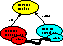
\includegraphics[width=150px]{Images/fig2.pdf} \hspace{1cm}

\includegraphics[width=150px]{Images/fig3.pdf} \\
\begin{itemize}
	\item Encapsulation des données, boite noire
	\item Un objet permet de regrouper en une seule entité et de façon indissociable données et procédures d'exploitation.
	\item Un objet est une instance de classe 
		\begin{itemize}
			\item ses données sont les variables d'instance, attributs variables, données membres. Les données sont accessibles uniquement à traver les procédures (programmation par état) $\rightarrow$ c'est rémanent (ie si l'objet se modifie lors d'une procédure, alors l'état initial n'est pas restauré). \\
			Remarque : En Java, l'unité d'encapsulation est la classe (les objets d'une même classe peuvent accéder aux champs privés des autres instances de la même classe). Ca devrait être l'objet.
			\item Les procédures sont les méthodes, attributs procédures, fonctions membres. Il y a des méthodes exportées (elles définissent l'interface) et des méthodes cachées (utiles uniquement à l'implémentation)
		\end{itemize}
\end{itemize}

\titre{Programmation par état :}
	\begin{itemize}
		\item On travaille par référence et non par valeur
		\item En java, les types primitifs passent par valeur
	\end{itemize}

\titre{Exemple :} Processus
\begin{itemize}
	\item Que \titre{fait} un processus ?
	\begin{itemize}	
		\item Suspendre
		\item Réveiller
		\item Priorité
	\end{itemize}
	\item Qu'\titre{est} un processus ? 
	\begin{itemize}
		\item Ressources
		\item Contexte
		\item Programme
	\end{itemize}
	\item $\rightarrow$ Ces deux points de vue peuvent être mixés par l'héritage multiple, mais nous en général on choisira une des deux approches et on s'y tiendra.
\end{itemize}
